% Documento de memoria para proyecto academico de analitica Big Data.
% Basado en una plantilla LaTeX adaptada para la asignatura.

\documentclass[12pt]{report}

% Paquetes LaTeX y estilos globales
\input{etc/pkgs}
\input{etc/style}

%%%%%%%%%%%%%%%%%%%%%%%%%%%%%%%%%%%%%%%%%%%%%%%%%%%%%%%%%%%%%%%%%%%%%%%%%%%%%%%%%%%%%

% Variables para la portada
\setTitle{Analisis escalable de movilidad urbana con Apache Spark y Apache Zeppelin sobre datos masivos de taxis de Nueva York}
\setAuthor{Pablo Vargas Sáez \\ Manuel López Pavía \\ GR71} % Si hay más de un autor, separarlos con \\
%%%%%%%%%%%%%%%%%%%%%%%%%%%%%%%%%%%%%%%%%%%%%%%%%%%%%%%%%%%%%%%%%%%%%%%%%%%%%%%%%%%%%

% Dedicatoria del trabajo
% Si no se desea incluir, comentar o borrar la línea siguiente para eliminar la página de dedicatoria
% \setDedication{Aqui la dedicatoria del trabajo}

%%%%%%%%%%%%%%%%%%%%%%%%%%%%%%%%%%%%%%%%%%%%%%%%%%%%%%%%%%%%%%%%%%%%%%%%%%%%%%%%%%%%%

% Comienzo del documento
\begin{document}

    % Portada y secciones no numeradas
    \thispagestyle{empty} % Impide que se incluya número de página en la portada
\begin{center}

\vspace*{1cm}


\includegraphics[width=\textwidth]{figures/etsii_us.png}

\vspace*{3cm}
\begin{large}
\end{large}

\vspace*{0.1in}
\textbf{\huge \tfgTitle}

\vspace*{.2in}

\vspace*{3cm}

\vspace*{0.2in}

\vspace*{0.2in}

\vspace*{.6in}

{\large Realizado por}\\
\textbf{\Large \tfgAuthors}



\end{center}

% Dedicatoria
\ifdefined\tfgDedication
    \newpage
    \thispagestyle{empty}
    
    \vspace*{\fill}
    \begin{center}
    \textit{\tfgDedication}
    \end{center}
    \vspace*{\fill}
\fi

\clearpage\setcounter{page}{1} % Comienza a incluir números de página a partir de aquí
\pagenumbering{roman} % En números romanos
    \chapter*{Resumen}
Este proyecto de la asignatura Complementos de Bases de Datos desarrolla una solución
de analítica de datos masivos para movilidad urbana utilizando el conjunto de viajes de
taxi de Nueva York (\textit{NYC Taxi \& Limousine Commission}, Yellow Taxi).
La implementación integra Apache Spark como motor de procesamiento distribuido,
Apache Zeppelin como entorno de análisis interactivo y Python/PySpark para
enriquecimiento geográfico y visualización con mapas.

La aportación central es un flujo completo y reproducible: carga de ficheros Parquet,
limpieza trazable con reglas explícitas, enriquecimiento temporal y geográfico, y
ejecución de consultas analíticas en dos notebooks de Zeppelin. El primero,
\texttt{Análisis Taxis Nueva York.zpln}, concentra la carga, el preprocesamiento y
todos los análisis tabulares y gráficos. El segundo,
\texttt{Análisis Taxis Nueva York Mapas.zpln}, consume los indicadores exportados
por zona y genera mapas coropléticos interactivos con Folium.

Entre los hallazgos principales, el análisis muestra picos de actividad en franjas de
tarde-noche, un volumen claramente dominante de viajes estándar frente a viajes a
aeropuerto, y contrastes muy marcados entre distritos en velocidad media, tarifa y
equilibrio de flujos de movilidad.

Como limitaciones, el despliegue se realiza en infraestructura local y no en clúster
productivo. Aun así, la arquitectura deja preparada la migración a entornos más
escalables (Spark Standalone, YARN o Kubernetes) sin rehacer la lógica analítica.

\vspace{.5cm}

\textbf{Palabras clave:} Big Data, Apache Spark, Apache Zeppelin, PySpark, Parquet,
movilidad urbana, Spark SQL, analítica urbana, calidad del dato, Folium.
    
    % Índice del documento y de figuras
    \begingroup
        % Los enlaces son normalmente azules, pero en los índices se configuran a negro para que no aparezca todo azul
        \hypersetup{linkcolor=black}
        \tableofcontents
        \listoffigures
        \listoftables
        \lstlistoflistings{}
    \endgroup
    
    % Cambia el estilo de números de página de romanos a normal
    \clearpage\pagenumbering{arabic}
    
    % Capítulos del trabajo
    \chapter{Introducción}\label{cap:introduccion}

\section{Contexto y motivación}
La movilidad urbana genera volúmenes de datos que exceden las capacidades de
procesamiento tradicional. En este escenario, Apache Spark se ha consolidado como una
tecnología de referencia para analítica distribuida por su modelo de ejecución y su
optimización de consultas \cite{zaharia2012resilient,armbrust2015sparksql,sparkdocs}.
Para la exploración interactiva y la comunicación de resultados, Apache Zeppelin aporta
un formato notebook que integra código, consultas y visualizaciones en un único flujo
de trabajo \cite{zeppelindocs}.

El presente trabajo aplica este stack al conjunto de datos público de la
\textit{New York City Taxi and Limousine Commission} (NYC TLC), centrado en registros
Yellow Taxi en formato Parquet \cite{nyctlc,nyctlcparquet,parquetdocs}. El interés no
es únicamente técnico: se busca demostrar cómo convertir datos masivos de viajes en
evidencia analítica clara para apoyar decisiones sobre patrones de demanda, coste y
comportamiento temporal de la movilidad.

Además, se adopta una arquitectura reproducible en entorno local con Docker, de forma
que cualquier miembro del equipo pueda replicar la ejecución y validar resultados sin
dependencias manuales difíciles de mantener \cite{dockerdocs}.

\section{Objetivos}
\subsection{Objetivo general}
Diseñar e implementar un sistema analítico Big Data reproducible y defendible,
capaz de procesar, limpiar, enriquecer, consultar y visualizar datos masivos de
viajes de taxi en Nueva York, culminando en notebooks de Zeppelin que
concentran todo el análisis técnico y las visualizaciones geográficas.

\subsection{Objetivos específicos}
\begin{itemize}
	\item Cargar y validar ficheros Yellow Taxi en formato Parquet dentro del
	entorno Spark.
	\item Definir y aplicar reglas trazables de calidad del dato directamente
	en los notebooks de Zeppelin.
	\item Generar variables derivadas para análisis temporal, geográfico y económico.
	\item Integrar Spark SQL y DataFrames para consultas analíticas reproducibles.
	\item Enriquecer geográficamente los datos mediante GeoJSON de zonas TLC.
	\item Exportar indicadores por zona a CSV para alimentar mapas coropléticos.
	\item Construir visualizaciones geográficas interactivas con Folium.
\end{itemize}

\section{Alcance}
El alcance funcional del proyecto incluye:
\begin{itemize}
	\item Ejecución local con Docker Compose y servicios Spark + Zeppelin.
	\item Carga, limpieza y enriquecimiento de datos Yellow Taxi (enero 2025).
	\item Análisis temporal y geográfico-económico en notebooks interactivos.
	\item Exportación de indicadores por zona para mapas coropléticos con Folium.
	\item Generación de mapas interactivos que permitan inspección por zona.
\end{itemize}

Quedan fuera del alcance:
\begin{itemize}
	\item Despliegue productivo en clúster empresarial multiusuario.
	\item Orquestación avanzada (por ejemplo, Airflow) y monitorización completa.
	\item Validación con datos de múltiples años de forma exhaustiva en infraestructura
	de alta disponibilidad.
\end{itemize}

Este recorte de alcance es intencional y coherente con el contexto docente: prioriza
calidad técnica, trazabilidad y capacidad de defensa frente a complejidad operativa.

\section{Contribuciones del trabajo}
Las contribuciones principales son las siguientes:
\begin{itemize}
	\item \textbf{Flujo analítico integrado en Zeppelin}: dos notebooks que cubren
	desde la carga hasta la visualización geográfica, sin scripts externos.
	\item \textbf{Criterios de calidad explícitos}: reglas concretas para filtrar registros
	inconsistentes y justificar su impacto.
	\item \textbf{Enriquecimiento geográfico completo}: uso de GeoJSON y Folium para
	representar indicadores por zona TLC con mapas coropléticos interactivos
	\cite{foliumdocs,geojsonspec}.
	\item \textbf{Exportación de indicadores por zona}: generación de CSVs de métricas
	agregadas por origen y destino para alimentar visualizaciones externas.
	\item \textbf{Narrativa defendible}: documentación técnica que conecta decisiones,
	implementación y resultados sin introducir métricas inventadas.
\end{itemize}

\section{Estructura del documento}
El documento se organiza en siete capítulos principales. Tras esta introducción,
el Capítulo 2 describe el estudio previo y la gestión del trabajo. El Capítulo 3
formaliza los requisitos y el análisis del problema. El Capítulo 4 presenta el
diseño de la arquitectura y del flujo analítico. El Capítulo 5 detalla la implementación
real del repositorio y los notebooks de Zeppelin. El Capítulo 6 recoge
las pruebas de validación funcional y técnica. Por último, el capítulo de
conclusiones resume logros, limitaciones y líneas de trabajo futuro.


    \chapter{Estudio previo y gestión del trabajo}\label{cap:gestion}

\section{Introducción}
Este capítulo describe cómo se planificó y gobernó el trabajo para llegar a un
resultado técnico completo sin perder trazabilidad. La gestión se orientó a un
objetivo claro: construir una solución reproducible en entorno local, con notebooks
versionados, decisiones justificadas y una narrativa defendible en presentación.

\section{Contexto tecnológico de partida}
La selección tecnológica se apoyó en herramientas abiertas y ampliamente adoptadas
en analítica de datos:
\begin{itemize}
	\item Apache Spark para procesamiento distribuido y consultas analíticas.
	\item Apache Zeppelin para desarrollo exploratorio, análisis y visualización.
	\item Docker Compose para estandarizar el entorno entre miembros del equipo.
	\item Python/PySpark para enriquecimiento geográfico y generación de mapas
	con Folium.
\end{itemize}

La elección de Parquet como formato de entrada permitió mantener coherencia entre
eficiencia de almacenamiento y rendimiento de lectura en consultas analíticas.
Los indicadores por zona se exportan a CSV para su consumo en visualizaciones
geográficas.

\section{Metodología de trabajo}
Se aplicó un enfoque incremental con entregables verificables en cada iteración.
Cada bloque cerraba con una revisión técnica de tres aspectos: viabilidad,
reproducibilidad y claridad documental.

\begin{enumerate}
	\item \textbf{Iteración 1 - Base de ejecución}: estructura de repositorio,
	dockerización y arranque de servicios.
	\item \textbf{Iteración 2 - Carga y limpieza}: notebook principal con carga
	de Parquet, reglas de calidad y enriquecimiento.
	\item \textbf{Iteración 3 - Análisis}: consultas temporales, geográficas y
	económicas en el notebook principal.
	\item \textbf{Iteración 4 - Visualización geográfica}: exportación de CSVs
	por zona y notebook de mapas con Folium.
	\item \textbf{Iteración 5 - Cierre académico}: pruebas, documentación y
	conclusiones.
\end{enumerate}

Este enfoque permitió controlar el alcance y detectar pronto bloqueos técnicos,
evitando una integración tardía de componentes.

\section{Planificación funcional}
La planificación final se alineó con los dos notebooks de Zeppelin y los
artefactos de datos:

\begin{table}[H]
	\centering
	\caption{Planificación por bloques funcionales}
	\begin{tabular}{|p{2.3cm}|p{4.7cm}|p{6.4cm}|}
		\hline
		\textbf{Bloque} & \textbf{Objetivo} & \textbf{Entregable principal} \\
		\hline
		B1 & Ingesta y validación & Carga de Parquet y validación de esquema \\
		\hline
		B2 & Calidad del dato & Reglas de limpieza + dataset limpio en memoria \\
		\hline
		B3 & Análisis temporal & Consultas por hora, día y franja horaria \\
		\hline
		B4 & Análisis geográfico-económico & Join con GeoJSON + indicadores por zona \\
		\hline
		B5 & Exportación de indicadores & CSVs por zona de origen y destino \\
		\hline
		B6 & Mapas interactivos & Notebook de mapas coropléticos con Folium \\
		\hline
	\end{tabular}
\end{table}

\section{Gestión de riesgos}
Durante el trabajo se identificaron riesgos recurrentes en proyectos Big Data
académicos y se definieron respuestas preventivas.

\begin{table}[H]
	\centering
	\caption{Riesgos relevantes y medidas de mitigación}
	\begin{tabular}{|p{4.0cm}|p{3.2cm}|p{6.2cm}|}
		\hline
		\textbf{Riesgo} & \textbf{Impacto} & \textbf{Mitigación aplicada} \\
		\hline
		Memoria insuficiente en local & Alto & Análisis centrado en un mes (enero 2025) y ajuste de parámetros Spark \\
		\hline
		Inconsistencia entre entornos del equipo & Alto & Uso de Docker Compose y comandos estandarizados \\
		\hline
		Resultados difíciles de defender & Medio & Reglas de limpieza explícitas y trazabilidad de salidas \\
		\hline
		Dependencia de datos auxiliares geográficos & Medio & Generación de GeoJSON desde shapefile con script auxiliar \\
		\hline
		Sobrecarga documental al final & Medio & Redacción continua por iteraciones y cierre por capítulo \\
		\hline
	\end{tabular}
\end{table}

\section{Recursos y estimación de esfuerzo}
El proyecto se desarrolló en contexto docente, por lo que no se imputan licencias
de software. La estimación económica se centra en esfuerzo de equipo y coste operativo
del entorno local.

\begin{table}[H]
	\centering
	\caption{Estimación orientativa de esfuerzo y coste}
	\begin{tabular}{|p{6.8cm}|c|c|}
		\hline
		\textbf{Concepto} & \textbf{Cantidad} & \textbf{Coste estimado (EUR)} \\
		\hline
		Esfuerzo técnico del equipo (análisis, código y documentación) & 120 h & 0 \\
		\hline
		Software y licencias (Spark, Zeppelin, Python, Docker) & -- & 0 \\
		\hline
		Infraestructura cloud & -- & 0 \\
		\hline
		Consumo eléctrico y uso de equipos locales & -- & 20 \\
		\hline
		\textbf{Total estimado} & -- & \textbf{20} \\
		\hline
	\end{tabular}
\end{table}

\section{Conclusiones}
La gestión del trabajo permitió mantener equilibrio entre ambición técnica y alcance
realista. El resultado no es un prototipo aislado, sino una solución completa con
notebooks de análisis y mapas, exportación de indicadores y documentación coherente,
preparada para presentación académica y para evolución futura a entornos de mayor
escala.
    \chapter{Análisis del problema}\label{cap:analisis}

\section{Introducción}
En este capítulo se formaliza el problema desde la perspectiva de ingeniería de
datos: qué información se necesita, qué funcionalidades debe cumplir el sistema,
y qué restricciones garantizan que los resultados sean técnicamente defendibles.

El objetivo no es construir un producto comercial, sino una solución académica
completa, reproducible y trazable, capaz de convertir datos masivos de viajes en
evidencia analítica útil.

\section{Preguntas de análisis que guían el proyecto}
El sistema se diseñó para responder, al menos, las siguientes preguntas:
\begin{itemize}
	\item ¿Cómo se distribuye la demanda de viajes por franja horaria y día de semana?
	\item ¿Qué zonas concentran mayor volumen de recogidas y destinos?
	\item ¿Qué diferencias económicas aparecen por zona (tarifa, propina, ingreso)?
	\item ¿Existe un desequilibrio territorial entre recogidas y destinos por distrito?
	\item ¿Cómo difiere el comportamiento de viajes estándar frente a viajes de aeropuerto?
\end{itemize}

Estas preguntas se reflejan directamente en los notebooks de Zeppelin, que actúan
como pieza de síntesis del trabajo.

\section{Requisitos de información}
Los datos base proceden del repositorio público de NYC TLC
(\textit{Yellow Taxi Trip Records}) \cite{nyctlc,nyctlcparquet}. La fuente principal
se consume en formato Parquet por su adecuación a cargas analíticas
\cite{parquetdocs}.

Campos mínimos utilizados:
\begin{itemize}
	\item \texttt{tpep\_pickup\_datetime}, \texttt{tpep\_dropoff\_datetime};
	\item \texttt{passenger\_count}, \texttt{trip\_distance};
	\item \texttt{PULocationID}, \texttt{DOLocationID};
	\item \texttt{payment\_type}, \texttt{fare\_amount}, \texttt{tip\_amount},
	\texttt{total\_amount};
	\item \texttt{VendorID}, \texttt{RatecodeID}, \texttt{store\_and\_fwd\_flag}.
\end{itemize}

Datos geográficos auxiliares:
\begin{itemize}
	\item Shapefile de zonas TLC, convertido a GeoJSON para enriquecer y visualizar
	por \texttt{LocationID}.
\end{itemize}

\section{Requisitos funcionales}
\textbf{RF-01. Carga de datos Parquet.} El sistema debe cargar el fichero
\texttt{yellow\_tripdata\_2025-01.parquet} en Spark y validar su esquema.

\textbf{RF-02. Procesamiento distribuido.} El sistema debe cargar y transformar los
datos con Apache Spark en modo distribuido local.

\textbf{RF-03. Limpieza trazable.} El sistema debe aplicar reglas explícitas sobre
nulos, duración, distancia, importes, pasajeros y coherencia temporal.

\textbf{RF-04. Variables derivadas.} El sistema debe generar variables para análisis
temporal (fecha, hora, día, franja horaria) y operativo (duración, velocidad).

\textbf{RF-05. Traducción de códigos.} El sistema debe convertir codificación numérica
(vendor, pago, tarifa, flag) a etiquetas legibles de negocio.

\textbf{RF-06. Integración geográfica.} El sistema debe enriquecer el dataset por
zonas de origen y destino usando el GeoJSON de zonas TLC.

\textbf{RF-07. Consultas analíticas.} El sistema debe ejecutar consultas por hora,
franja, tipo de viaje, pasajeros, distrito y balance territorial.

\textbf{RF-08. Exportación de indicadores por zona.} El sistema debe generar CSVs de
indicadores (viajes, tarifa, propina, distancia, duración, ingresos, hora pico/valle)
por zona de origen y de destino.

\textbf{RF-09. Visualización geográfica.} El sistema debe generar mapas coropléticos
interactivos con Folium, con inspección por tooltip.

\textbf{RF-10. Trazabilidad de ejecución.} El sistema debe ofrecer salidas verificables
en los notebooks y archivos de indicadores para su revisión posterior.

\section{Requisitos no funcionales}
\textbf{RNF-01. Reproducibilidad.} La ejecución debe replicarse entre equipos mediante
Docker Compose.

\textbf{RNF-02. Claridad técnica.} Notebooks y documentación deben ser
comprensibles para revisión académica.

\textbf{RNF-03. Trazabilidad.} Cada fase del flujo debe dejar evidencias de salida
(recuento de limpieza, indicadores exportados y visualizaciones generadas).

\textbf{RNF-04. Escalabilidad conceptual.} La solución local debe permitir justificar
una migración futura a clúster real.

\textbf{RNF-05. Honestidad de resultados.} No se deben reportar métricas inventadas;
la discusión debe apoyarse en ejecuciones observables.

\textbf{RNF-06. Mantenibilidad.} El repositorio debe separar datos, notebooks y
documentación para facilitar evolución.

\section{Restricciones y supuestos}
\begin{itemize}
	\item El entorno de ejecución es local; por tanto, memoria y CPU son limitadas.
	\item El análisis se centra en un mes de referencia (enero de 2025) para
	mantener tiempos de procesamiento razonables.
	\item La calidad del dato depende de la fuente pública; el sistema no corrige
	errores semánticos externos no detectables por reglas objetivas.
	\item El GeoJSON de zonas se genera mediante un script auxiliar
	(\texttt{convert.py}) a partir del shapefile oficial de TLC.
\end{itemize}

\section{Criterios de aceptación}
Se consideran cumplidos los requisitos cuando:
\begin{itemize}
	\item el notebook principal ejecuta sus bloques de carga, limpieza y análisis
	sin errores;
	\item se obtienen los 14 ficheros CSV de indicadores por zona (7 de origen y
	7 de destino);
	\item el notebook de mapas genera visualizaciones coropléticas navegables;
	\item se documenta el flujo completo con evidencias de ejecución.
\end{itemize}

\section{Conclusiones}
El análisis confirma que el problema es abordable con un flujo de analítica
distribuida en Spark siempre que se mantengan tres principios: limpieza trazable,
reproducibilidad operativa y transparencia en la interpretación de resultados.
Con estos requisitos, los notebooks de Zeppelin se convierten en evidencia
integrada de implementación y análisis.
    \chapter{Diseño de la solución}\label{cap:diseno}

\section{Introducción}
El diseño persigue un equilibrio explícito entre tres objetivos: capacidad analítica,
reproducibilidad local y claridad para defensa académica. En lugar de una arquitectura
sobredimensionada, se adopta un diseño modular con separación entre datos, notebooks y
documentación, lo que permite ampliar componentes sin rehacer el núcleo del flujo
analítico.

\section{Arquitectura de alto nivel}
La solución se organiza en cuatro capas:

\begin{itemize}
	\item \textbf{Capa de ejecución}: contenedores \texttt{zeppelin},
	\texttt{spark-master} y \texttt{spark-worker-1} en Docker Compose.
	\item \textbf{Capa de datos}: directorio \texttt{data/} con el Parquet de
	entrada, CSVs de indicadores exportados, shapefile y GeoJSON de zonas.
	\item \textbf{Capa de procesamiento}: notebooks de Zeppelin con PySpark y
	Spark SQL para carga, limpieza, análisis y exportación.
	\item \textbf{Capa de visualización}: gráficas nativas de Zeppelin para
	análisis tabular y mapas coropléticos con Folium para análisis geográfico.
\end{itemize}

El uso de Spark en modo distribuido local permite conservar la semántica de un
procesamiento escalable, aun ejecutando en infraestructura docente.

\section{Diseño de almacenamiento y rutas}
El diseño físico de datos responde a un flujo directo:

\begin{itemize}
	\item \texttt{data/yellow\_tripdata\_2025-01.parquet}: fichero de entrada
	con los registros Yellow Taxi de enero de 2025.
	\item \texttt{data/taxi\_zones.*}: shapefile oficial de zonas TLC (5 ficheros).
	\item \texttt{data/nyc\_taxi\_zones.geojson}: GeoJSON generado a partir del
	shapefile mediante el script auxiliar \texttt{convert.py}.
	\item \texttt{data/*.csv}: indicadores por zona exportados desde Spark
	(14 ficheros: viajes, tarifa, propina, distancia, duración, ingresos y horas
	pico/valle, cada uno por origen y por destino).
\end{itemize}

Esta estructura plana es intencionada: todos los datos residen en un único directorio
montado como volumen Docker (\texttt{/data}), accesible tanto desde Spark como desde
Python.

\section{Diseño del flujo analítico}
El flujo se implementa íntegramente en dos notebooks de Zeppelin, sin scripts
externos de ETL:

\begin{enumerate}
	\item \textbf{Notebook principal}
	(\texttt{Análisis Taxis Nueva York.zpln}): concentra la carga del Parquet,
	la limpieza, el enriquecimiento y todas las consultas analíticas. Está
	organizado en bloques secuenciales que procesan los datos paso a paso.
	\item \textbf{Notebook de mapas}
	(\texttt{Análisis Taxis Nueva York Mapas.zpln}): lee los CSVs de indicadores
	exportados por el notebook principal y genera mapas coropléticos interactivos
	con Folium.
\end{enumerate}

Se incluye además una versión del notebook de mapas ya ejecutada
(\texttt{Análisis Taxis Nueva York Mapas (Ejecutados).zpln}), que permite revisar
las visualizaciones sin necesidad de volver a ejecutar el código.

En la fase de procesamiento se definen métricas derivadas clave:

\[
\text{trip\_duration\_minutes} =
\frac{\text{unix}(\texttt{dropoff}) - \text{unix}(\texttt{pickup})}{60}
\]

\[
\text{average\_speed\_mph} =
\frac{\texttt{trip\_distance}}{\text{trip\_duration\_minutes} / 60}
\]

Y se aplican restricciones de limpieza para eliminar registros no plausibles
(duraciones no positivas, velocidades extremas, importes negativos y nulos críticos).

\section{Diseño del notebook principal}
El notebook principal se diseña como un flujo integrado con párrafos Spark y
Spark SQL:

\begin{enumerate}
	\item Carga del Parquet de referencia y validación básica de esquema.
	\item Limpieza avanzada con filtros de dominio (rango de
	\texttt{LocationID}, pasajeros mínimos y coherencia temporal).
	\item Enriquecimiento geográfico mediante GeoJSON de zonas TLC.
	\item Traducción de códigos a etiquetas legibles (vendor, pago, tarifa, flag).
	\item Ejecución de consultas analíticas por hora, franja, tipo de viaje,
	pasajeros y balance entre recogidas y destinos.
	\item Exportación de indicadores agregados por zona a CSV.
	\item Generación de visualizaciones comparativas directamente en Zeppelin.
\end{enumerate}

Este diseño permite que el notebook sea simultáneamente entorno de análisis,
artefacto de demostración y evidencia de ejecución del proyecto.

\section{Diseño de consultas e indicadores}
Los indicadores extraídos se agrupan en cuatro vistas principales:

\begin{itemize}
\item \textbf{Comportamiento temporal}: viajes por hora, tarifa media y duración
media, además de comparativa de 1 de enero frente al resto del mes.
\item \textbf{Comparativas operativas}: diferencia entre viajes estándar y viajes
de aeropuerto en volumen, distancia, duración, tarifa y propina.
\item \textbf{Patrones geográficos}: métricas agregadas por distrito de recogida
(distancia, velocidad y coste por milla).
\item \textbf{Balance territorial}: contraste recogidas vs destinos por distrito
y su diferencia neta.
\end{itemize}

Los indicadores por zona se exportan a CSV con la siguiente estructura:
\begin{itemize}
\item \textbf{Por zona de origen (pickup)}: viajes, tarifa media, propina media,
distancia media, duración media, ingresos totales y hora pico/valle.
\item \textbf{Por zona de destino (dropoff)}: los mismos indicadores agregados por
\texttt{DOLocationID}.
\end{itemize}

Estos CSVs alimentan directamente el notebook de mapas, cerrando el ciclo
análisis-visualización.

\section{Decisiones de diseño y trade-offs}
Las decisiones más relevantes fueron:

\begin{itemize}
	\item \textbf{Parquet como fuente principal}: mejora de I/O y lectura selectiva
	por columnas, adecuado para cargas analíticas con Spark.
	\item \textbf{CSV como formato de exportación}: los indicadores por zona se
	exportan a CSV para su consumo por Folium/Pandas, que requiere formatos
	tabulares simples. No se usa CSV como formato de almacenamiento analítico.
	\item \textbf{Zeppelin como interfaz única}: facilita defensa al unir código,
	salida, gráficas y explicación en el mismo documento.
	\item \textbf{Dos notebooks separados}: el análisis principal se mantiene
	independiente de la visualización geográfica, permitiendo ejecutar uno sin
	el otro y reduciendo el acoplamiento.
	\item \textbf{Consultas SQL centradas en interpretación}: se priorizan métricas
	que aportan lectura de movilidad real frente a tablas excesivamente técnicas.
\end{itemize}

Como trade-off, se renuncia a complejidad de producción (autoscaling,
alta disponibilidad y orquestación externa) para mantener foco académico.

\section{Conclusiones}
El diseño implementado es coherente con el alcance del proyecto de asignatura y con
la naturaleza del dataset. La separación en dos notebooks, junto con la exportación
de indicadores por zona, proporciona una base sólida para análisis reproducible hoy y
para evolución a despliegues más escalables en el futuro.
    \chapter{Implementación}\label{cap:implementacion}

\section{Introducción}
Este capítulo describe la implementación real del proyecto a nivel de repositorio,
notebooks y artefactos de datos. El objetivo es mostrar cómo el diseño del
capítulo anterior se materializa en entregables ejecutables y verificables.

\section{Herramientas y versiones}
Las herramientas principales utilizadas son:
\begin{itemize}
	\item \textbf{Apache Spark 3.5.1} para procesamiento distribuido.
	\item \textbf{Apache Zeppelin 0.11.1} para notebooks y visualización integrada.
	\item \textbf{Python 3 + PySpark} para enriquecimiento geográfico y mapas.
	\item \textbf{Folium} para generación de mapas coropléticos interactivos.
	\item \textbf{Docker Compose} para levantar servicios en local.
	\item \textbf{Git/GitHub} para control de versiones y trazabilidad.
\end{itemize}

Dependencias Python adicionales instaladas en el contenedor:
\begin{itemize}
	\item \texttt{geopandas}, \texttt{pyogrio} (para convertir shapefile a GeoJSON)
	\item \texttt{folium} (para mapas coropléticos)
	\item \texttt{numpy<2}, \texttt{pyarrow} (compatibilidad de datos)
\end{itemize}

\section{Estructura implementada}
El repositorio final se organiza de la siguiente forma:
\begin{itemize}
	\item \texttt{data/}: Parquet de entrada, shapefile, GeoJSON generado,
	script auxiliar \texttt{convert.py} y los 14 CSVs de indicadores exportados.
	\item \texttt{notebooks/}: los dos notebooks de Zeppelin (análisis principal
	y mapas) más una versión del notebook de mapas ya ejecutada.
	\item \texttt{docs/}: memoria LaTeX y documentación del proyecto.
	\item \texttt{logs/}: directorio de logs de Zeppelin.
\end{itemize}

\section{Orquestación con Docker Compose}
La ejecución local utiliza tres servicios:
\begin{itemize}
	\item \texttt{zeppelin}: interfaz notebook en el puerto \texttt{8080}.
	\item \texttt{spark-master}: coordinador Spark en \texttt{7077},
	con interfaz web en \texttt{8081}.
	\item \texttt{spark-worker-1}: nodo de cómputo con 3 GB de memoria
	y 2 núcleos.
\end{itemize}

Los volúmenes Docker montan \texttt{./data} como \texttt{/data} dentro de los
contenedores, de forma que tanto Spark como Python acceden al mismo directorio
de datos. Esta topología mantiene coherencia con un esquema distribuido real,
pero con complejidad controlada para entorno académico.

\section{Script auxiliar: generación de GeoJSON}
El único script fuera de los notebooks es \texttt{data/convert.py}, que convierte
el shapefile de zonas TLC a GeoJSON:

\begin{lstlisting}[language=python,caption={Script de conversión shapefile a GeoJSON}]
import geopandas as gpd
import pandas as pd

gdf = gpd.read_file('/data/taxi_zones.shp')
gdf = gdf.to_crs(epsg=4326)
gdf.to_file('/data/nyc_taxi_zones.geojson', driver='GeoJSON')
\end{lstlisting}

Se ejecuta una única vez dentro del contenedor Zeppelin:
\begin{lstlisting}[language=bash,caption={Ejecución del script de conversión}]
docker exec -u root -it zeppelin bash -c \
  "/opt/conda/envs/python_3_with_R/bin/python3 /data/convert.py"
\end{lstlisting}

\section{Implementación de los notebooks de Zeppelin}
El entregable analítico principal consta de dos notebooks:
\begin{itemize}
	\item \texttt{Análisis Taxis Nueva York.zpln}: notebook principal con carga,
	limpieza, análisis y exportación de indicadores.
	\item \texttt{Análisis Taxis Nueva York Mapas.zpln}: notebook de visualización
	geográfica con mapas coropléticos Folium.
\end{itemize}

Adicionalmente, se incluye \texttt{Análisis Taxis Nueva York Mapas (Ejecutados).zpln},
una versión del notebook de mapas ya ejecutada que permite revisar los resultados
visuales sin necesidad de relanzar el código.

\subsection{Notebook principal: flujo de análisis}

\subsection{Fase 1: carga y validación}
Se carga \texttt{/data/yellow\_tripdata\_2025-01.parquet}, se imprime esquema,
se cuenta el volumen de registros y se inspecciona una muestra inicial.

\subsection{Fase 2: limpieza y enriquecimiento en Spark}
En el notebook se aplican filtros de dominio adicionales, incluyendo:

\begin{itemize}
	\item \texttt{PULocationID} y \texttt{DOLocationID} en rango válido (1..263);
	\item pasajeros mínimos mayores o iguales a 1;
	\item tarifas e importes positivos;
	\item año de recogida esperado (2025);
	\item \texttt{dropoff} posterior a \texttt{pickup}.
\end{itemize}

También se traduce codificación numérica a etiquetas legibles de negocio para
\texttt{vendor}, tipo de pago, tarifa y bandera \texttt{store\_and\_fwd}.

\subsection{Fase 3: enriquecimiento geográfico}
Se lee \texttt{/data/nyc\_taxi\_zones.geojson}, se explota el array de
\texttt{features} y se realizan joins para añadir atributos de zona de recogida y
destino. Tras el enriquecimiento, se registra la vista temporal
\texttt{dfFinal} para consultas SQL.

\subsection{Fase 4: consultas de análisis y resultados}
Sobre la vista \texttt{dfFinal} se ejecutan consultas que sintetizan el
comportamiento del mes de enero de 2025. Los resultados se organizan en siete
bloques temáticos que cubren temporalidad, geografía, economía y tipología de
viaje.

\subsubsection*{a) Patrón horario de actividad}
La distribución horaria de viajes revela un patrón coherente con los ciclos de
actividad urbana de una gran metrópolis. La Figura~\ref{fig:ny-trips-hour}
muestra una curva con forma de campana asimétrica:
\begin{itemize}
\item el mínimo absoluto se registra a las 04:00 con apenas 12{,}175 viajes,
correspondiente al periodo de menor actividad urbana;
\item la demanda crece de forma sostenida a partir de las 06:00, coincidiendo con
el inicio de la jornada laboral y los desplazamientos al trabajo;
\item el máximo se alcanza a las 17:00 con 205{,}245 viajes, momento que
coincide con la salida generalizada del trabajo;
\item a las 18:00 el volumen apenas desciende (204{,}191 viajes), lo que indica
una hora punta prolongada, típica de ciudades con alta densidad de servicios.
\end{itemize}

Este patrón tiene implicaciones directas: sugiere que la oferta de vehículos
debería concentrarse entre las 15:00 y las 19:00 para cubrir la máxima demanda,
mientras que en madrugada la sobreoferta podría generar ineficiencia operativa.

\begin{figure}[H]
\centering
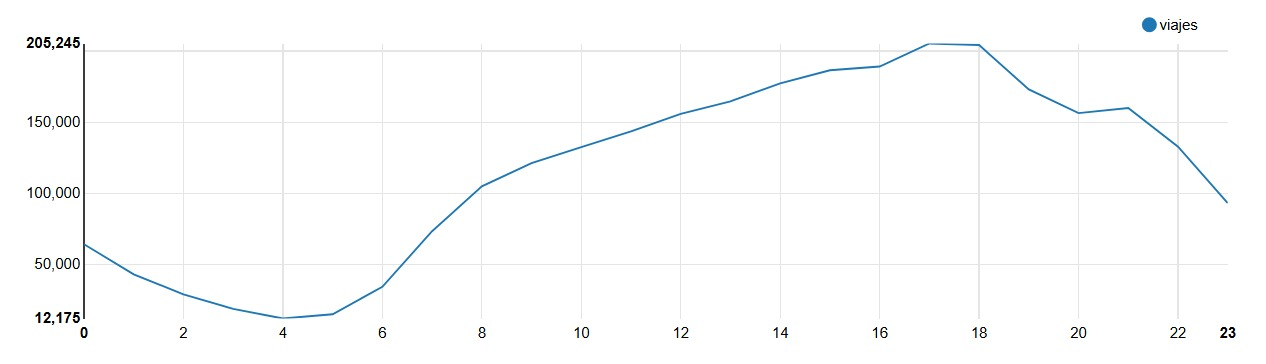
\includegraphics[width=0.95\textwidth]{figures/ny_trips_by_hour.jpeg}
\caption{Viajes por hora de recogida en enero de 2025. Se observa el mínimo
a las 04:00 (12{,}175) y el máximo a las 17:00 (205{,}245).}
\label{fig:ny-trips-hour}
\end{figure}

La Figura~\ref{fig:ny-fare-duration-hour} complementa el análisis anterior
al superponer tarifa media y duración media por hora. Se observa que:
\begin{itemize}
\item la tarifa media presenta un pico notable a las 05:00 (26.46 USD),
explicable porque los viajes de madrugada tienden a ser más largos (por ejemplo,
trayectos nocturnos desde zonas de ocio al aeropuerto o a periferia);
\item entre las 09:00 y las 13:00 aparece un segundo máximo de duración
(hasta 22.84 min a las 12:00), posiblemente asociado a congestión en hora
intermedia;
\item durante la franja de mayor demanda (17:00--18:00), la tarifa media se
estabiliza en torno a 18 USD con duraciones de unos 14 minutos, lo que refleja
viajes cortos pero frecuentes.
\end{itemize}

\begin{figure}[H]
\centering
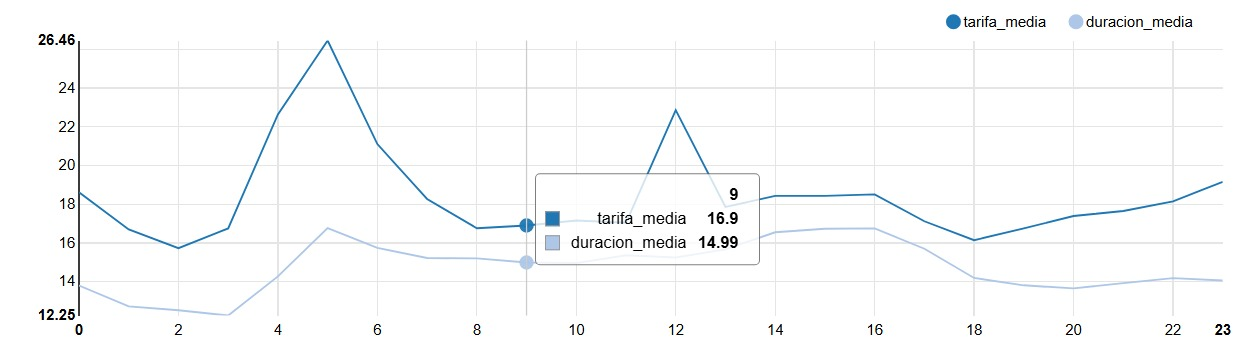
\includegraphics[width=0.95\textwidth]{figures/ny_fare_duration_by_hour.jpeg}
\caption{Tarifa media y duración media por hora de recogida. El pico de tarifa
a las 05:00 (26.46 USD) se explica por viajes largos nocturnos.}
\label{fig:ny-fare-duration-hour}
\end{figure}

\subsubsection*{b) 1 de enero frente al resto del mes}
El 1 de enero es el principal festivo del año y su comportamiento difiere
sustancialmente del patrón habitual. La Figura~\ref{fig:ny-jan1-vs-rest}
compara la media de viajes por hora del 1 de enero frente al promedio diario
del resto del mes:
\begin{itemize}
\item durante la madrugada (00:00--04:00), el 1 de enero supera ampliamente al
resto: a las 00:00 registra 5{,}543 viajes frente a los 1{,}977 habituales,
un incremento del 180\%, explicado por las celebraciones de Año Nuevo;
\item ambas series convergen sobre las 05:00, donde se alcanza el mínimo común
(343 viajes en día 1);
\item a partir de las 08:00, el resto de días domina con claridad, alcanzando
un máximo de 6{,}709 viajes por día a las 17:00, frente a los 4{,}246 del
festivo.
\end{itemize}

Este contraste evidencia que los eventos extraordinarios alteran drásticamente
la distribución de demanda y refuerza la importancia de segmentar el análisis
temporal para no distorsionar métricas agregadas.

\begin{figure}[H]
\centering
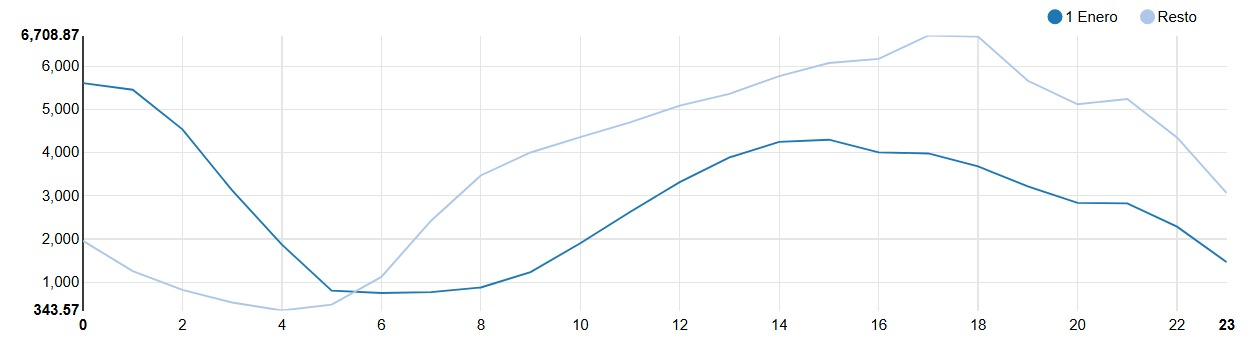
\includegraphics[width=0.98\textwidth]{figures/ny_jan1_vs_rest_by_hour.jpeg}
\caption{Media de viajes por hora: 1 de enero frente al promedio del resto
del mes. La madrugada del festivo muestra un comportamiento invertido respecto
al patrón diario normal.}
\label{fig:ny-jan1-vs-rest}
\end{figure}

\subsubsection*{c) Diferencias por distrito de recogida}
La Figura~\ref{fig:ny-borough-speed-cost} presenta indicadores operativos
agregados por distrito de recogida. Los contrastes son muy marcados:
\begin{itemize}
\item \textbf{Manhattan}: distancia media de solo 2.20 millas con velocidad
de 10.13 mph y un coste por milla de 6.50 USD. Los viajes cortos en zona
de alta congestión explican la baja velocidad y el elevado coste relativo.
\item \textbf{Queens}: 12.54 millas de media con 22.35 mph y 4.43 USD por
milla. Su proximidad a los aeropuertos JFK y LaGuardia genera viajes más
largos y rápidos.
\item \textbf{Bronx}: la mayor distancia media (17.03 millas) y la mayor
velocidad (22.28 mph), con el coste por milla más bajo (2.12 USD), lo que
refleja recorridos por vías rápidas con menor congestión.
\item \textbf{EWR} (Newark Airport): con 77.67 USD de tarifa media, casi
5 veces superior a Manhattan, pero a 31.37 mph, mostrando el perfil típico
de traslado interurbano al aeropuerto de Nueva Jersey.
\end{itemize}

Estos datos confirman que la movilidad en taxi no es homogénea: cada distrito
tiene un perfil operativo distinto que afecta directamente a ingresos,
eficiencia y experiencia del pasajero.

\begin{figure}[H]
\centering
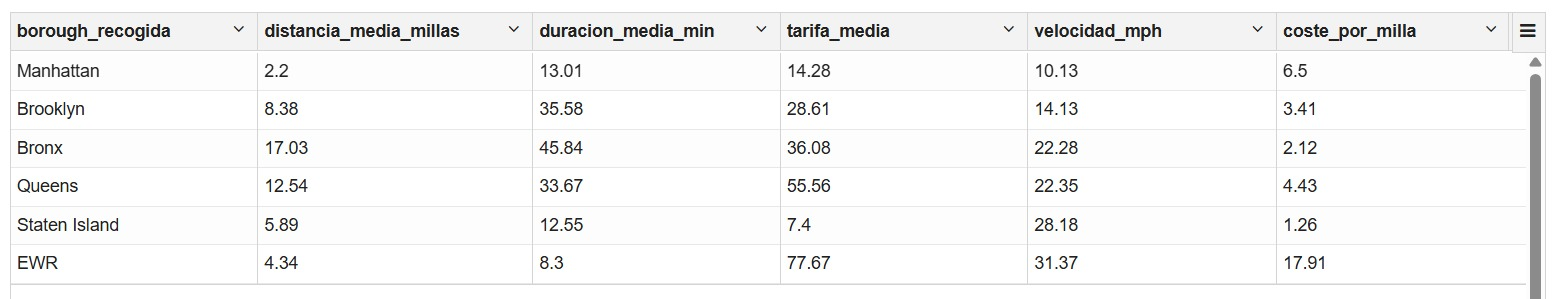
\includegraphics[width=0.95\textwidth]{figures/ny_borough_speed_cost.jpeg}
\caption{Indicadores operativos por distrito de recogida: distancia media,
duración, tarifa, velocidad y coste por milla.}
\label{fig:ny-borough-speed-cost}
\end{figure}

\subsubsection*{d) Viajes estándar vs aeropuerto}
La Figura~\ref{fig:ny-trip-type} compara los dos grandes segmentos de
servicio. Las diferencias son significativas en todos los indicadores:
\begin{itemize}
\item los viajes estándar dominan en volumen (2{,}696{,}555 frente a 94{,}614
de aeropuerto, ratio 28.5:1);
\item sin embargo, el viaje medio a aeropuerto recorre 17.71 millas frente a
2.65 (6.7 veces más), dura 44.66 minutos frente a 13.99 y genera una tarifa
media de 70.88 USD frente a 16.10;
\item la propina media de aeropuerto (11.91 USD) triplica la estándar
(3.18 USD), posiblemente porque el pasajero valora más un servicio puerta a
puerta con equipaje;
\item el porcentaje de propina es similar (16.8\% vs 19.7\%), lo que indica
que la diferencia en propina absoluta se debe a la mayor tarifa base, no a un
comportamiento más generoso.
\end{itemize}

\begin{figure}[H]
\centering
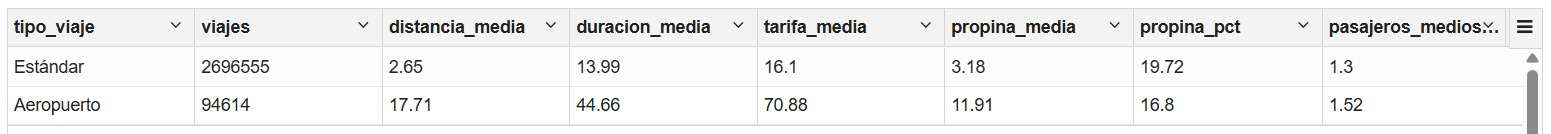
\includegraphics[width=0.92\textwidth]{figures/ny_trip_type_comparison.jpeg}
\caption{Comparativa entre viajes estándar y de aeropuerto: volumen, distancia,
duración, tarifa, propina y pasajeros medios.}
\label{fig:ny-trip-type}
\end{figure}

\subsubsection*{e) Franjas horarias y tipo de semana}
Para capturar la interacción entre momento del día y tipo de jornada, se
definieron cuatro franjas horarias: mañana (6--12h), tarde (12--18h), noche
(18--23h) y madrugada (23--6h). La Figura~\ref{fig:ny-timeslot-weektype}
muestra los resultados por viajes por día:
\begin{itemize}
\item la \textbf{tarde} es la franja dominante tanto en laborables
(35{,}066 viajes/día) como en fin de semana (33{,}678), con diferencia
mínima entre ambos;
\item la \textbf{mañana} presenta la mayor brecha: los laborables superan al
fin de semana en un 51\% (21{,}000 vs 14{,}000 viajes/día), reflejando los
desplazamientos al trabajo;
\item la \textbf{noche} muestra también más actividad en laborables
(28{,}000 vs 23{,}000), posiblemente por vuelta a casa tras jornada laboral;
\item la \textbf{madrugada} es la única franja donde el fin de semana supera
a los laborables (14{,}000 vs 6{,}000), consecuencia directa del ocio nocturno.
\end{itemize}

\begin{figure}[H]
\centering
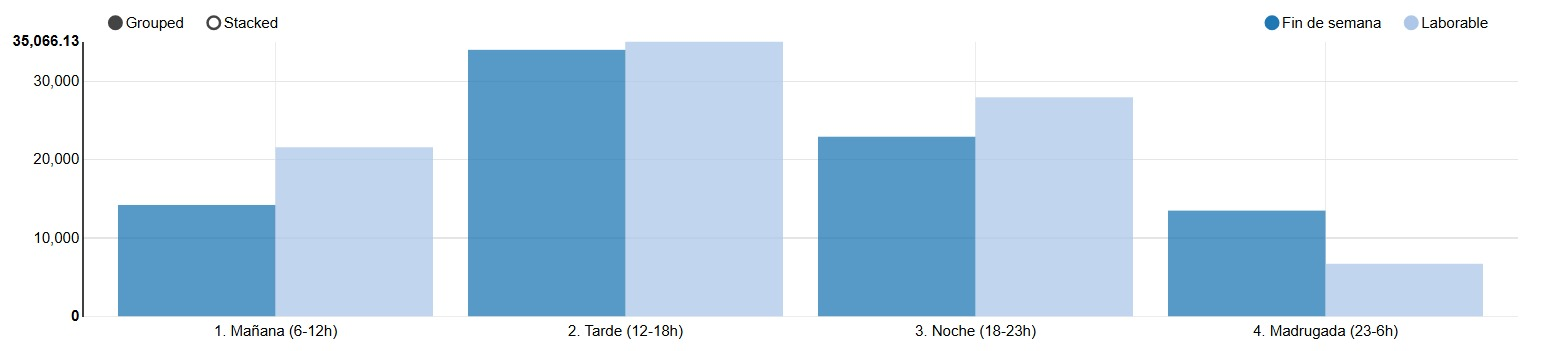
\includegraphics[width=0.95\textwidth]{figures/ny_timeslot_weektype.jpeg}
\caption{Viajes por día según franja horaria y tipo de semana. La madrugada es
la única franja donde el fin de semana supera a los laborables.}
\label{fig:ny-timeslot-weektype}
\end{figure}

\subsubsection*{f) Número de pasajeros}
La Figura~\ref{fig:ny-passengers} desglosa el servicio por ocupación del
vehículo. Los hallazgos son claros:
\begin{itemize}
\item los viajes de \textbf{1 pasajero} representan el 79\% del total
(2{,}231{,}648 registros), con tarifa media de 17.50 USD;
\item con \textbf{2 pasajeros} se registran 389{,}587 viajes (13.8\%),
y la tarifa media sube a 19.87 USD, lo que sugiere viajes ligeramente más
largos compartidos;
\item de 3 a 6 pasajeros el volumen desciende progresivamente (86{,}800,
53{,}995, 17{,}327 y 11{,}805 respectivamente), pero la tarifa media aumenta
hasta 21.38 USD para 4 pasajeros;
\item la propina media se mantiene estable entre 2.92 y 3.68 USD
independientemente de la ocupación, lo que indica que no se ajusta al número
de beneficiarios del servicio;
\item la distancia media es también estable (entre 2.92 y 3.68 millas),
lo que descarta que viajes con más pasajeros sean sistemáticamente más largos.
\end{itemize}

\begin{figure}[H]
\centering
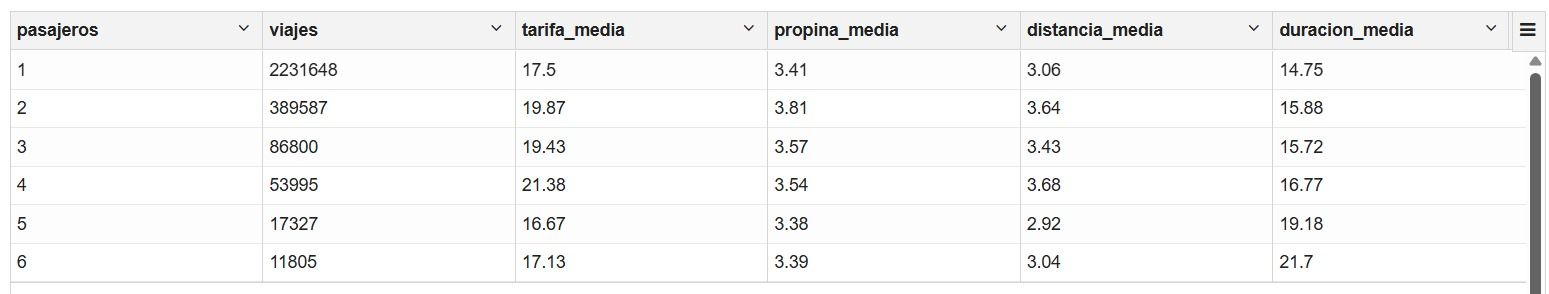
\includegraphics[width=0.95\textwidth]{figures/ny_passengers_trips_fare.jpeg}
\caption{Volumen de viajes, tarifa media, propina, distancia y duración
según número de pasajeros.}
\label{fig:ny-passengers}
\end{figure}

\subsubsection*{g) Balance recogidas-destinos por distrito}
La dinámica territorial se estudia mediante dos visualizaciones complementarias.
La Figura~\ref{fig:ny-pickup-vs-dest} muestra el porcentaje relativo de
recogidas frente a destinos por distrito, mientras que la
Figura~\ref{fig:ny-balance-borough} presenta la diferencia neta.

Los resultados revelan desequilibrios territoriales significativos:
\begin{itemize}
\item \textbf{Queens} es el mayor emisor neto con +119{,}591 viajes
(más recogidas que destinos), consistente con su función de acceso
aeroportuario: los taxis recogen pasajeros que aterrizan y los llevan a
Manhattan u otros distritos;
\item \textbf{Brooklyn} es el mayor receptor neto con -81{,}809 viajes,
indicando que recibe más viajes de los que genera, posiblemente por
desplazamientos residenciales de vuelta desde Manhattan;
\item \textbf{Manhattan} muestra un ligero déficit (-27{,}000 aprox.),
sorprendente dado su papel central, pero explicable porque el alto volumen
de recogidas y destinos casi se compensa;
\item \textbf{EWR} presenta un fuerte desequilibrio porcentual
(1.5\% de recogidas vs 98.99\% de destinos), lógico para un aeropuerto
donde predominan las llegadas en taxi;
\item \textbf{Staten Island} muestra un patrón similar con predominancia
clara de destinos (89\%) sobre recogidas (10\%).
\end{itemize}

\begin{figure}[H]
\centering
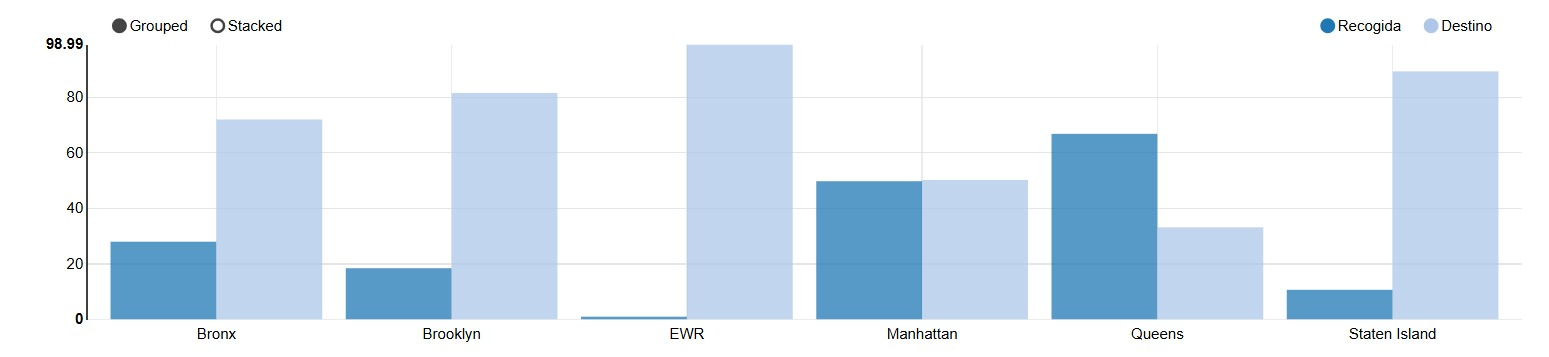
\includegraphics[width=0.95\textwidth]{figures/ny_pickup_vs_destination_by_borough.jpeg}
\caption{Proporción de recogidas frente a destinos por distrito. EWR y
Staten Island muestran los mayores desequilibrios relativos.}
\label{fig:ny-pickup-vs-dest}
\end{figure}

\begin{figure}[H]
\centering
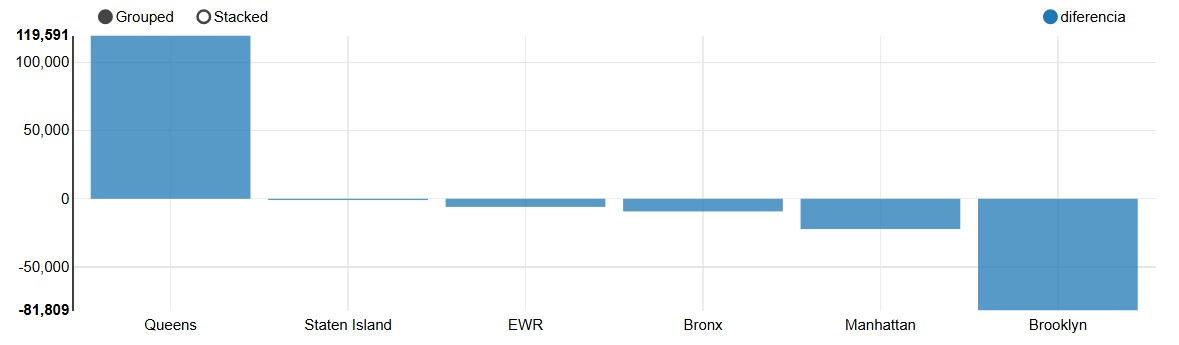
\includegraphics[width=0.95\textwidth]{figures/ny_pickup_destination_balance.jpeg}
\caption{Diferencia neta entre recogidas y destinos por distrito. Queens
como emisor neto (+119{,}591) y Brooklyn como receptor neto (-81{,}809).}
\label{fig:ny-balance-borough}
\end{figure}

\subsection{Fase 5: interpretación consolidada}
La secuencia de consultas y gráficas permite construir una lectura integrada del
servicio de taxi en Nueva York que articula cuatro dimensiones de análisis:

\begin{itemize}
	\item \textbf{Demanda temporal}: la actividad sigue ciclos predecibles
	(mínimo a las 04:00, máximo a las 17:00), con alteraciones claras en
	festivos y fines de semana.
	\item \textbf{Heterogeneidad espacial}: cada distrito tiene un perfil
	operativo propio en velocidad, distancia y coste, condicionado por
	infraestructura viaria y función urbana.
	\item \textbf{Segmentación de servicio}: los viajes a aeropuerto,
	aunque minoritarios en volumen, generan tarifas e ingresos por viaje
	muy superiores al servicio estándar.
	\item \textbf{Dinámica origen-destino}: los flujos no son simétricos;
	existen distritos emisores netos (Queens) y receptores netos
	(Brooklyn), lo que refleja patrones reales de movilidad residencial y
	funcional.
\end{itemize}

Adicionalmente, para cada zona TLC se exportaron indicadores detallados tanto
por origen como por destino:
\begin{itemize}
	\item \textbf{Origen (pickup)}: viajes, tarifa media, propina media,
	distancia media, duración media, viajes hora pico/valle e ingresos totales.
	\item \textbf{Destino (dropoff)}: mismos indicadores agregados por
	\texttt{DOLocationID}.
\end{itemize}

Esta separación permite comparar la dinámica de entrada y salida de cada zona
a nivel granular, más allá de la agregación por distrito.

\section{Artefactos de salida}
Tras ejecutar el flujo completo, los artefactos generados son:

\begin{itemize}
	\item \textbf{Datos de entrada}: \texttt{data/yellow\_tripdata\_2025-01.parquet}
	\item \textbf{GeoJSON generado}: \texttt{data/nyc\_taxi\_zones.geojson}
	\item \textbf{Indicadores por zona de origen} (7 CSVs):
	\texttt{viajes\_por\_zona.csv}, \texttt{tarifa\_por\_zona.csv},
	\texttt{propina\_por\_zona.csv}, \texttt{distancia\_por\_zona.csv},
	\texttt{duracion\_por\_zona.csv}, \texttt{ingresos\_por\_zona.csv},
	\texttt{viajes\_hora\_pico.csv}
	\item \textbf{Indicadores por zona de destino} (7 CSVs):
	\texttt{viajes\_por\_destino.csv}, \texttt{tarifa\_por\_destino.csv},
	\texttt{propina\_por\_destino.csv}, \texttt{distancia\_por\_destino.csv},
	\texttt{duracion\_por\_destino.csv}, \texttt{ingresos\_por\_destino.csv},
	\texttt{viajes\_hora\_valle.csv}
	\item \textbf{Mapas interactivos}: generados en HTML dentro del notebook
	de mapas con Folium.
\end{itemize}

\section{Conclusiones}
La implementación alcanzada cubre de extremo a extremo el caso de uso planteado:
ingesta de Parquet, calidad del dato, enriquecimiento geográfico, análisis
tabular, exportación de indicadores y visualización con mapas interactivos.
Los notebooks de Zeppelin no actúan como pruebas aisladas, sino como síntesis
operativa de todo el proyecto y base directa para defensa oral.
    \chapter{Pruebas}\label{cap:pruebas}

\section{Introducción}
El objetivo de este capítulo es documentar cómo se validó la solución de forma
pragmática en entorno local. Las pruebas cubren el flujo completo: ingesta,
limpieza, enriquecimiento, exportación de indicadores y visualización final en
los notebooks de Zeppelin.

\section{Estrategia de validación}
Se aplicaron tres tipos de verificación:

\begin{itemize}
	\item \textbf{Pruebas funcionales de flujo}: comprobar que cada etapa produce la
	salida esperada y habilita la siguiente.
	\item \textbf{Pruebas de consistencia de datos}: verificar reglas de limpieza y
	coherencia temporal/numérica tras los filtros.
	\item \textbf{Pruebas de presentación analítica}: confirmar que los notebooks
	ejecutan correctamente y generan gráficas, indicadores y mapas interpretables.
\end{itemize}

\section{Pruebas funcionales del notebook principal}
El notebook \texttt{Análisis Taxis Nueva York.zpln} se utilizó como prueba
integrada de extremo a extremo. Los párrafos principales registrados aparecen
con estado \texttt{FINISHED} y código de ejecución \texttt{SUCCESS}.

\begin{table}[H]
	\centering
	\caption{Pruebas funcionales sobre el notebook principal}
	\begin{tabular}{|p{1.7cm}|p{6.1cm}|p{4.1cm}|p{2.4cm}|}
		\hline
		\textbf{ID} & \textbf{Caso de prueba} & \textbf{Evidencia esperada} & \textbf{Resultado} \\
		\hline
		PF-01 & Carga de Parquet y revisión de esquema & Conteo de registros y muestra de filas & Superada \\
		\hline
		PF-02 & Limpieza de registros con reglas de dominio & Dataset limpio cacheado y recuento final & Superada \\
		\hline
		PF-03 & Join geográfico con GeoJSON & Columnas de zona origen/destino en dataset final & Superada \\
		\hline
		PF-04 & Consulta horaria de viajes/tarifa/duración & Tabla de 24 horas generada en Zeppelin & Superada \\
		\hline
		PF-05 & Comparativas por tipo de viaje y pasajeros & Tablas agregadas sin errores de ejecución & Superada \\
		\hline
		PF-06 & Balance recogida-destino por distrito & Tabla de diferencias por borough generada & Superada \\
		\hline
		PF-07 & Exportación de CSVs de indicadores por zona & 14 ficheros CSV generados en \texttt{/data} & Superada \\
		\hline
	\end{tabular}
\end{table}

\section{Pruebas funcionales del notebook de mapas}
El notebook \texttt{Análisis Taxis Nueva York Mapas.zpln} se validó tras la
ejecución del notebook principal, que genera los CSVs de indicadores necesarios.

\begin{table}[H]
	\centering
	\caption{Pruebas funcionales sobre el notebook de mapas}
	\begin{tabular}{|p{1.7cm}|p{6.1cm}|p{4.1cm}|p{2.4cm}|}
		\hline
		\textbf{ID} & \textbf{Caso de prueba} & \textbf{Evidencia esperada} & \textbf{Resultado} \\
		\hline
		PM-01 & Lectura de CSVs de indicadores & DataFrames cargados sin errores & Superada \\
		\hline
		PM-02 & Carga del GeoJSON de zonas & GeoDataFrame con geometrías válidas & Superada \\
		\hline
		PM-03 & Generación de mapas coropléticos & Mapas Folium renderizados con tooltips & Superada \\
		\hline
		PM-04 & Inspección interactiva por zona & Tooltip con nombre de zona e indicador al pasar el ratón & Superada \\
		\hline
	\end{tabular}
\end{table}

\section{Validación de resultados analíticos}
Además de validar ejecución, se comprobó que los resultados clave del notebook son
coherentes entre sí y con la lógica de negocio.

\begin{itemize}
\item En la serie horaria, el mínimo de viajes aparece a las 04:00 (12{,}175) y el
máximo a las 17:00 (205{,}245), patrón consistente con movilidad urbana real.
\item La comparación 1 de enero vs resto del mes confirma un comportamiento anómalo
de madrugada en el festivo, sin romper coherencia en el resto de franjas.
\item La tipología de viaje refleja dominio de viajes estándar
(2{,}696{,}555) frente a aeropuerto (94{,}614), con mayor distancia y tarifa en este
último caso.
\item El balance territorial (recogidas - destinos) identifica a Queens como emisor
neto (+119{,}591) y a Brooklyn como receptor neto (-81{,}809), en línea con una
dinámica centro-periferia esperable.
\item Los 14 CSVs exportados contienen datos coherentes con las consultas del notebook
y sirven como entrada verificable para los mapas.
\end{itemize}

\section{Pruebas sobre reglas de calidad del dato}
Se verificó que las reglas implementadas en Spark son coherentes con el dominio
del problema y se aplican de forma explícita. En particular:

\begin{itemize}
	\item no se admiten fechas de recogida o entrega nulas;
	\item la duración del viaje debe ser positiva;
	\item distancia e importes deben ser positivos;
	\item el orden temporal \texttt{dropoff > pickup} es obligatorio;
	\item la velocidad media debe estar dentro de umbrales plausibles;
	\item \texttt{PULocationID} y \texttt{DOLocationID} deben estar en rango
	válido (1..263).
\end{itemize}

Como resultado, el flujo elimina registros inconsistentes antes de calcular
indicadores, reduciendo el riesgo de conclusiones erróneas.

\section{Pruebas de coherencia entre notebooks}
Se verificó que la cadena de dependencia entre notebooks funciona correctamente:

\begin{itemize}
	\item El notebook principal genera los 14 CSVs en \texttt{/data}.
	\item El notebook de mapas los lee y genera visualizaciones sin errores.
	\item Los valores mostrados en los tooltips de los mapas son consistentes
	con las tablas del notebook principal.
	\item La versión ejecutada del notebook de mapas mantiene las salidas
	correctas para revisión posterior.
\end{itemize}

\section{Limitaciones de las pruebas}
Las validaciones realizadas son suficientes para el alcance docente, pero presentan
limitaciones reconocidas:

\begin{itemize}
	\item no se ejecutó una batería sistemática de estrés en varios nodos físicos;
	\item la variabilidad de hardware local puede afectar tiempos absolutos;
	\item no se incluyó automatización CI/CD de pruebas de regresión completas.
\end{itemize}

Estas limitaciones no invalidan los hallazgos, pero delimitan su interpretación.

\section{Conclusiones}
Las pruebas confirman que la solución funciona de extremo a extremo: ambos notebooks
ejecutan correctamente sus bloques principales, las reglas de limpieza son coherentes,
los CSVs exportados alimentan correctamente los mapas, y las salidas generadas permiten
justificar resultados analíticos de manera trazable. Con ello, la implementación queda
validada para su defensa académica.
    \chapter{Conclusiones}\label{cap:conclusiones}

\section{Síntesis del trabajo realizado}
Este proyecto ha desarrollado una solución analítica completa para estudiar movilidad
urbana con datos masivos de taxis de Nueva York, combinando Spark, Zeppelin y
Python/PySpark en un entorno local reproducible. El resultado no se limita a un
notebook aislado: se ha construido un flujo técnico coherente que integra ingesta
de Parquet, calidad del dato, análisis tabular y gráfico, exportación de indicadores
por zona y visualización geográfica con mapas interactivos.

\section{Cumplimiento de objetivos}
Los objetivos definidos en la introducción se consideran alcanzados:
\begin{itemize}
	\item se cargó y validó el dataset de enero 2025 en formato Parquet;
	\item se implementó limpieza trazable con criterios explícitos y defendibles;
	\item se generaron variables derivadas para análisis temporal y económico;
	\item se ejecutaron consultas analíticas en Spark SQL y DataFrames;
	\item se enriquecieron los datos geográficamente con GeoJSON de zonas TLC;
	\item se exportaron 14 CSVs de indicadores por zona de origen y destino;
	\item se construyeron dos notebooks de Zeppelin: uno con análisis completo
	y otro con mapas coropléticos interactivos con Folium.
\end{itemize}

\section{Valor técnico y académico}
El valor principal del trabajo reside en su equilibrio entre ingeniería y
comunicación de resultados:
\begin{itemize}
	\item desde el punto de vista técnico, el flujo es reproducible con Docker y
	fácilmente extensible a más meses o datasets;
	\item desde el punto de vista académico, los notebooks permiten defender
	decisiones de diseño con evidencia ejecutable;
	\item desde el punto de vista metodológico, se mantuvo trazabilidad entre
	requisitos, implementación y pruebas;
	\item la separación en dos notebooks (análisis + mapas) facilita la
	reutilización y la presentación modular del trabajo.
\end{itemize}

\section{Limitaciones}
Se reconocen limitaciones inherentes al alcance elegido:
\begin{itemize}
	\item infraestructura local con recursos acotados;
	\item ausencia de despliegue productivo con alta disponibilidad;
	\item análisis limitado a un único mes (enero 2025), que puede no
	reflejar patrones estacionales completos.
\end{itemize}

Estas limitaciones son compatibles con el objetivo del proyecto y no comprometen la
validez de las conclusiones dentro del contexto definido.

\section{Líneas de trabajo futuro}
Como evolución natural del proyecto se proponen:
\begin{itemize}
	\item ampliar el periodo temporal analizado con más meses y temporadas completas;
	\item desplegar el flujo en un clúster real (Standalone, YARN o Kubernetes);
	\item incorporar orquestación de pipelines y pruebas automáticas de regresión;
	\item añadir capas de análisis predictivo (por ejemplo, demanda por franja horaria);
	\item construir un panel interactivo operativo para consumo no técnico;
	\item incluir una comparativa de rendimiento formal entre Parquet y CSV con
	infraestructura controlada.
\end{itemize}

\section{Cierre}
La solución final demuestra que es posible construir, con herramientas abiertas y
en un entorno docente, un sistema de analítica Big Data robusto y defendible.
Los notebooks de Zeppelin actúan como artefactos de síntesis del proyecto y dejan
una base sólida para continuar hacia escenarios de mayor escala y complejidad.


    \chapter{Declaración de uso de Inteligencia Artificial}\label{cap:uso-ia}

De acuerdo con las directrices de la asignatura, se declara de forma transparente
el uso de herramientas de inteligencia artificial generativa durante el desarrollo
de este proyecto.

\section{Generación del código}
La mayor parte del código del proyecto (notebooks de Zeppelin, configuración
Docker y scripts auxiliares) ha sido generada con asistencia de \textbf{Claude}
(Anthropic), un modelo de lenguaje conversacional. Esta decisión se tomó por
la falta de experiencia previa del equipo con las tecnologías específicas del
stack (PySpark, Spark SQL, Folium, GeoJSON).

No obstante, \textbf{todo el código ha sido revisado, comprendido y validado
por los autores} antes de su incorporación al proyecto. Las decisiones de
diseño, la selección de consultas y la estructura del flujo analítico
responden a criterios propios del equipo.

La conversación utilizada para la generación del código está disponible en el
siguiente enlace:

\begin{center}
\url{https://claude.ai/share/231f84af-d261-4aad-b579-fa9fdaf06f2e}
\end{center}

\section{Redacción de la memoria}
La memoria LaTeX ha sido desarrollada con asistencia del IDE
\textbf{Antigravity} (Google DeepMind), que integra un asistente de IA para
edición de código y documentación. Dado que Antigravity es una herramienta
local de escritorio, \textbf{no existe posibilidad de compartir o exportar
el historial de conversación} de la misma forma que con un chatbot web.

La IA se ha utilizado en parte para:
\begin{itemize}
    \item estructurar y redactar las secciones de la memoria;
    \item desarrollar los análisis textuales de las gráficas y darles un
    significado más profundo en el contexto de movilidad urbana;
    \item mantener coherencia entre capítulos y asegurar que la documentación
    refleja fielmente el estado real del repositorio.
\end{itemize}

En todos los casos, el trabajo se ha realizado \textbf{bajo supervisión
directa de los autores}, que han dirigido, corregido y aprobado cada
modificación.

\section{Decisiones propias del equipo}
Es importante destacar que las siguientes decisiones son \textbf{íntegramente
de los autores}, sin intervención de la IA:

\begin{itemize}
    \item la \textbf{elección de las gráficas} incluidas en la memoria, que
    han sido seleccionadas por considerarlas las más interesantes y
    representativas del análisis;
    \item los \textbf{contenidos y temas analizados}, elegidos por su
    conveniencia y relevancia para responder a las preguntas de movilidad
    planteadas;
    \item la \textbf{arquitectura del proyecto} (Docker + Spark + Zeppelin),
    propuesta por el equipo docente y adaptada por los autores;
    \item la \textbf{interpretación final de los resultados} y las conclusiones
    extraídas del análisis.
\end{itemize}

\section{Compromiso de honestidad}
Los autores asumen la responsabilidad íntegra sobre el contenido del proyecto
y la memoria. El uso de herramientas de IA ha sido un medio para acelerar el
desarrollo, no un sustituto del criterio técnico y académico propio.


    % Bibliografía
    \bibliographystyle{unsrtnat}
    \bibliography{bibliografia.bib}
        

% Fin del documento
\end{document}
